\documentclass{article}
\usepackage[margin=1in]{geometry}
\usepackage{problemset}
\showsolntrue

% Custom commands
\newcommand{\R}{\mathbb{R}}
\newcommand{\X}{\mathcal{X}}
\newcommand{\Y}{\mathcal{Y}}
\newcommand{\E}{\mathbb{E}}
\newcommand{\V}{\text{Var}}
\renewcommand{\P}{\mathbb{P}}
\DeclareMathOperator*{\argmax}{arg\,max}

\begin{document}

\pstitle{%
    DSC 140A%
}{
    Homework 4%
}[due Friday, December 5 at 11:59PM]

\begin{probset}
% Problem 1
\begin{prob}
    \textit{\textcolor{blue}{\textbf{Motivation:} In this problem, we'll explore the decision rule from LDA. Our goal is to highlight connections between the decision boundary from LDA and the linear models we've covered earlier in the course.}}

    Consider a classification dataset with $n$ points $(x_i, c_i)$ where $x_i \in \R^d$ is a feature vector and $c_i$ is a class label $c_i \in \{1, 2\}$. In what follows, we denote the number of points where $c_i = 1$ and $c_i = 2$ as $n_1$ and $n_2$, respectively.

    \begin{subprobset}
        % Subproblem 1.1
        \begin{subprob}
            Show that the LDA rule classifies to class 2 if and only if
            \[
                x^\top \hat{\Sigma}^{-1} (\hat{\mu}_2 - \hat{\mu}_1) > \frac{1}{2} (\hat{\mu}_2 + \hat{\mu}_1)^\top \hat{\Sigma}^{-1} (\hat{\mu}_2 - \hat{\mu}_1) - \log \frac{n_2}{n_1}
            \]

            \begin{soln}
                From slide 12 of lecture 13, we know that $c(x) = \text{argmax}_c p_c(x)\frac{n_c}{n}$. This means that we predict class 2 if and only if
                \begin{align}
                    p_2(x) \frac{n_2}{n} &> p_1(x) \frac{n_1}{n} \\
                    p_2(x) \frac{n_2}{n_1} &> p_1(x) \\
                    - \frac{1}{2} (x - \hat{\mu}_2)^\top \hat\Sigma^{-1} (x - \hat{\mu}_2) + \log \frac{n_2}{n_1} &> - \frac{1}{2} (x - \hat{\mu}_1)^\top \hat\Sigma^{-1} (x - \hat{\mu}_1) \\
                    \frac{1}{2} (x - \hat{\mu}_1)^\top \hat\Sigma^{-1} (x - \hat{\mu}_1) + \log \frac{n_2}{n_1} &> \frac{1}{2} (x - \hat{\mu}_2)^\top \hat\Sigma^{-1} (x - \hat{\mu}_2) \\
                    \frac{1}{2} ( \hat{\mu}_1^\top \hat\Sigma^{-1} \hat{\mu}_1 - 2x^\top\hat\Sigma^{-1} \hat{\mu}_1 ) + \log \frac{n_2}{n_1} &> \frac{1}{2} (\hat{\mu}_2^\top \hat\Sigma^{-1} \hat{\mu}_2 - 2x^\top\hat\Sigma^{-1} \hat{\mu}_2) \\
                    \frac{1}{2} ( 2x^\top\hat\Sigma^{-1} \hat{\mu}_2 - 2x^\top\hat\Sigma^{-1} \hat{\mu}_1 ) + \log \frac{n_2}{n_1} &> \frac{1}{2} (\hat{\mu}_2^\top \hat\Sigma^{-1} \hat{\mu}_2 - \hat{\mu}_1^\top \hat\Sigma^{-1} \hat{\mu}_1 ) \\
                    x^\top \hat{\Sigma}^{-1} (\hat{\mu}_2 - \hat{\mu}_1) &> \frac{1}{2} (\hat{\mu}_2 + \hat{\mu}_1)^\top \hat{\Sigma}^{-1} (\hat{\mu}_2 - \hat{\mu}_1) - \log \frac{n_2}{n_1}
                \end{align}
                From (4) to (5), we apply the distributive property of matrix multiplication and use the fact that $\hat{\Sigma}^{-1}$ is symmetric so $x^\top \hat{\Sigma}^{-1} \hat\mu = \hat\mu^\top \hat{\Sigma}^{-1} x$. From (6) to (7), we use difference of squares to simplify the expression.
            \end{soln}
        \end{subprob}

        % Subproblem 1.2
        \begin{subprob}
            Show that the rule shown above can be expressed as a linear classification model of the form:
            \[ c(x) = 2 \Leftrightarrow w^\top_{LDA} x + b_{LDA} \geq 0 \]

            \begin{soln}
                From above we know that \( c(x) = 2 \Leftrightarrow x^\top \hat{\Sigma}^{-1} (\hat{\mu}_2 - \hat{\mu}_1) > \frac{1}{2} (\hat{\mu}_2 + \hat{\mu}_1)^\top \hat{\Sigma}^{-1} (\hat{\mu}_2 - \hat{\mu}_1) - \log \frac{n_2}{n_1} \). This means that we can express the decision rule as a linear classification model of the form $w^\top_{LDA} x + b_{LDA} \geq 0$ where $w_{LDA} = \hat{\Sigma}^{-1} (\hat{\mu}_2 - \hat{\mu}_1)$ since the inner product is commutative and $b_{LDA} = \log \frac{n_2}{n_1} - \frac{1}{2} (\hat{\mu}_2 + \hat{\mu}_1)^\top \hat{\Sigma}^{-1} (\hat{\mu}_2 - \hat{\mu}_1)$ by moving the remaining terms to the left hand side. The only issue is that the inequality is not strictly greater than 0. However, this isn't an issue since we can choose to classify the border either way and here, we'll classify it as class 2.
            \end{soln}
        \end{subprob}
    \end{subprobset}
\end{prob}

\newpage
% Problem 2
\begin{prob}
    \textit{\textcolor{blue}{\textbf{Motivation:} In this problem, we'll work through a classification task using Quadratic Discriminant Analysis (QDA). We'll compute class-specific statistics, visualize the fitted distributions, and compare the resulting decision boundaries to those from LDA. Our goal is to give you hands-on practice with QDA, explore how it
    differs from LDA, and understand when and why these methods behave differently.}}

    Consider the following dataset with 12 points sampled from 3 classes:
    \begin{align*}
        y_i &= 0 : (0, 2), (2, 0), (5, 3), (-3, 5) \\
        y_i &= 1 : (\sqrt{2}, \sqrt{2}), (\sqrt{2}, \sqrt{2}), (4\sqrt{2}, -\sqrt{2}), (-4\sqrt{2}, -\sqrt{2}) \\
        y_i &= 2 : (3, 5), (1, 3), (8, 6), (0, -2)
    \end{align*}

    \begin{subprobset}
        % Subproblem 2.1
        \begin{subprob}
            Use the data above to compute the following estimates for each class $C \in \{0, 1, 2\}$:
            \begin{enumerate}
                \item $\mu_C$, the sample mean for class $C$
                \item $\Sigma_C$, the sample covariance matrix for class $C$
                \item $\pi_C$, the estimated probability that a point belongs to class $C$
            \end{enumerate}

            \begin{soln}
                First, $\pi_C = \frac{n_C}{n}$ and since $n_0 = n_1 = n_2 = 4$, $\pi_0 = \pi_1 = \pi_2 = \frac{1}{3}$. The work for the other values are found \href{https://www.desmos.com/3d/wxgbswgklq}{here}.
                \begin{itemize}
                    \item $\mu_0 = \frac{1}{4} \sum_{i=1}^4 x_i = (1, 2.5)$
                    \item $\mu_1 = \frac{1}{4} \sum_{i=1}^4 x_i = (\frac{1}{2}\sqrt{2}, 0)$
                    \item $\mu_2 = \frac{1}{4} \sum_{i=1}^4 x_i = (3, 3)$
                    
                    \item $\Sigma_0 = \frac{1}{3} \sum_{i=1}^4 (x_i - \mu_0)(x_i - \mu_0)^\top = \begin{pmatrix}
                        \frac{34}{3} & -\frac{10}{3} \\
                        -\frac{10}{3} & \frac{13}{3}
                    \end{pmatrix}$
                    \item $\Sigma_1 = \frac{1}{3} \sum_{i=1}^4 (x_i - \mu_1)(x_i - \mu_1)^\top = \begin{pmatrix}
                        22 & \frac{4}{3} \\
                        \frac{4}{3} & \frac{8}{3}
                    \end{pmatrix}$
                    \item $\Sigma_2 = \frac{1}{3} \sum_{i=1}^4 (x_i - \mu_2)(x_i - \mu_2)^\top = \begin{pmatrix}
                        \frac{38}{3} & 10 \\
                        10 & \frac{38}{3}
                    \end{pmatrix}$
                \end{itemize}
            \end{soln}
        \end{subprob}

        \newpage
        % Subproblem 2.2
        \begin{subprob}
            Sketch contour plots for the Normal distributions fitted by QDA. Your sketch should label the center of each distribution and depict the correct axis directions and relative axis lengths of isocontours.

            \begin{soln}
                \begin{center}
                    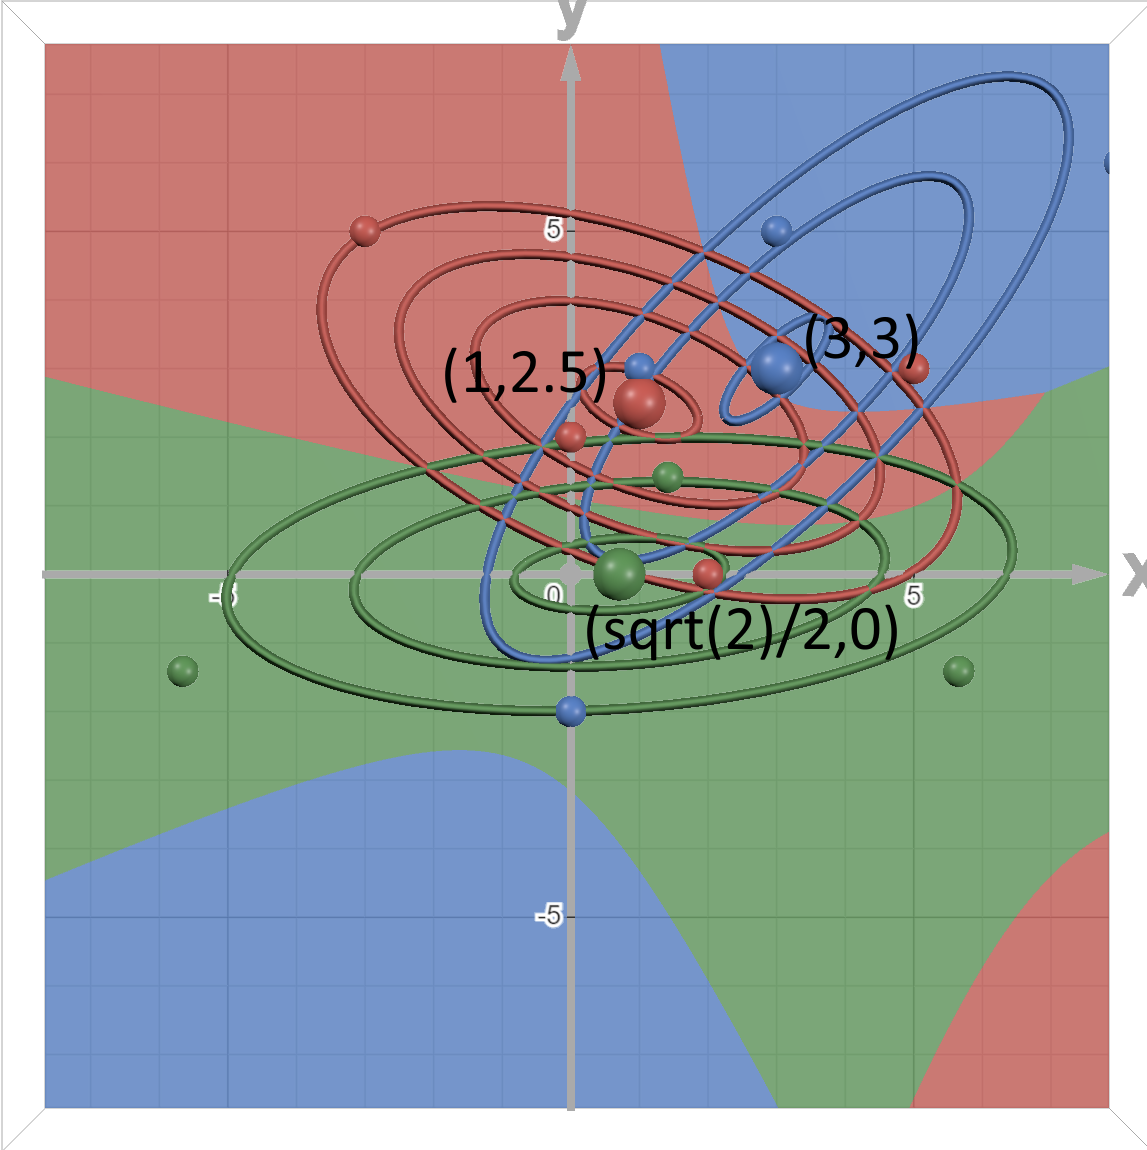
\includegraphics[width=0.6\textwidth]{Images/2.2.png}
                \end{center}
                Red is class 0, green is class 1, and blue is class 2.
            \end{soln}
        \end{subprob}

        % Subproblem 2.3
        \begin{subprob}
            Explain why you could not apply LDA to distinguish between the classes in Part (a)?

            \begin{soln}
                We would not be able to apply LDA to distinguish between the classes in Part (a) because the covariance matrices are not the same for all classes.
            \end{soln}
        \end{subprob}

        % Subproblem 2.4
        \begin{subprob}
            How could you re-frame your classification task to still run LDA?

            \begin{soln}
                We could re-frame our classification task to still run LDA by assuming that the population covariance matrices are the same for all classes. This would allow us to use the LDA decision rule to classify the points. For example, we can pool the covariance matrices of the three classes together using 
                \[
                    \hat\Sigma_{\text{pooled}}
                    = \frac{1}{\,n - K\,}
                    \sum_{C=0}^{K-1}
                    \sum_{i : y_i = C}
                    \bigl(x_i - \hat{\mu}_C\bigr)\bigl(x_i - \hat{\mu}_C\bigr)^\top.
                \] 
                to get a single covariance matrix $\hat{\Sigma}_{\text{pooled}}$ and then use the LDA decision rule to classify the points.
            \end{soln}
        \end{subprob}
    \end{subprobset}
\end{prob}

\newpage
% Problem 3
\begin{prob}
    \textit{\textcolor{blue}{\textbf{Motivation:} In this problem, we'll practice applying Naive Bayes to a simple dataset and explore how its assumptions affect predictions. We'll walk through basic probability computations, handle missing features, and examine how correlated or redundant features can violate the model's independence assumptions. Our goal is to understand how Naive Bayes works in practice and when its assumptions may break down.}}

    Consider a dataset where each point $(x_i, y_i)$ records a person's responses to a happiness survey.
    Each feature vector is $x_i = (rich, married, healthy)$, with binary values—for example, $x_i = (1, 0, 1)$ means the respondent is rich, not married, and healthy. The label is $y_i = 1$ if the person reports being happy. The dataset contains 8 points: 4 labeled $happy$ and 4 labeled $unhappy$, with the following feature vectors for each class:
    \begin{align*}
        happy : y_i &= 1 : (1, 1, 1), (0, 0, 1), (1, 1, 0), (1, 0, 1) \\
        unhappy : y_i &= 0 : (0, 0, 0), (1, 0, 0), (0, 0, 1), (0, 1, 0)
    \end{align*}
    Use the data above to estimate the following probabilities using Naive Bayes:

    \begin{subprobset}
        % Subproblem 3.1
        \begin{subprob}
            The probability that a person who is $not rich$ but $married$ and $healthy$ is $happy$?

            \begin{soln}
                \begin{align*}
                    \P(x=(0,1,1)\mid y=1) &= \P(r=0\mid1)\P(m=1\mid1)\P(h=1\mid1) = \frac14 \cdot \frac24 \cdot \frac34 = \frac{6}{64} \\
                    \P(x=(0,1,1)\mid y=0) &= \P(r=0\mid0)\P(m=1\mid0)\P(h=1\mid0) = \frac34 \cdot \frac14 \cdot \frac14 = \frac{3}{64} \\
                    \P(y=1\mid x = (0,1,1)) &= \frac{\P(x=(0,1,1)\mid y=1)\P(y=1)}{\P(x=(0,1,1)\mid y=1)\P(y=1) + \P(x=(0,1,1)\mid y=0)\P(y=0)} \\
                    &= \frac{\tfrac{6}{64}\tfrac{1}{2}}{\tfrac{6}{64}\tfrac{1}{2} + \tfrac{3}{64}\tfrac{1}{2}} = \frac23.
                \end{align*}
            \end{soln}
        \end{subprob}

        % Subproblem 3.2
        \begin{subprob}
            The probability that a person who is $not rich$ and $married$ is $happy$?

            \begin{soln}
                \begin{align*}
                    \P(x=(0,1,h)\mid y=1) &= \P(r=0\mid1)\P(m=1\mid1) = \frac14 \cdot \frac24 = \frac{2}{16} \\
                    \P(x=(0,1,h)\mid y=0) &= \P(r=0\mid0)\P(m=1\mid0) = \frac34 \cdot \frac14 = \frac{3}{16} \\
                    \P(y=1\mid x = (0,1,h)) &= \frac{\P(x=(0,1,h)\mid y=1)\P(y=1)}{\P(x=(0,1,h)\mid y=1)\P(y=1) + \P(x=(0,1,h)\mid y=0)\P(y=0)} \\
                    &= \frac{\frac{2}{16}\frac{1}{2}}{\frac{2}{16}\frac{1}{2} + \frac{3}{16}\frac{1}{2}} = \frac25.
                \end{align*}
            \end{soln}
        \end{subprob}

        % Subproblem 3.3
        \begin{subprob}
            Say we use a person's age to create three new binary features for each point:
            \[
            x_{i,4} = 1[age_i < 20] \quad
            x_{i,5} = 1[20 \leq age_i \leq 30] \quad
            x_{i,6} = 1[age_i > 30]
            \]
            Describe potential difficulties you may encounter by using Naive Bayes with these attributes.

            \begin{soln}
                We may encounter difficulties by using Naive Bayes with these attributes because the attributes are mutually exclusive and perfectly correlated. For example, if you know that $x_{i,4} = 1$, then $x_{i,5} = 0$ and $x_{i,6} = 0$. This means that the attributes are not independent and the conditional independence of Naive Bayes assumption is violated.
            \end{soln}
        \end{subprob}

        % Subproblem 3.4
        \begin{subprob}
            Given a classification task with $d$ binary features $x = (x_1, \ldots, x_d) \in \{0, 1\}^d$, let:
            \begin{align*}
                p_0 &= Pr(y = 0) &&
                w^0_j = Pr(x_j = 1 \mid y = 0) \\
                p_1 &= Pr(y = 1) &&
                w^1_j = Pr(x_j = 1 \mid y = 1)
            \end{align*}
            Show that a Naive Bayes decision rule to predict $\hat{y} = 1$ can be written in the form $w^\top x + b > 0$,
            where $w$ and $b$ are functions of $p_0, p_1, w^0_j, w^1_j$.

            \begin{soln}
                \begin{align*}
                    f(x) = \argmax_{y\in\{0,1\}} \P(y\mid x) \implies P(y=1\mid x) &> P(y=0\mid x) \\
                    \frac{\P(x \mid y = 1)\P(y=1)}{\P(x)} &> \frac{\P(x \mid y = 0)\P(y=0)}{\P(x)} \\
                    \P(x \mid y = 1)\P(y=1) &> \P(x \mid y = 0)\P(y=0) \\
                    p_1 \prod_{j=1}^d (w^1_j)^{x_j} (1 - w^1_j)^{1 - x_j} &> p_0 \prod_{j=1}^d (w^0_j)^{x_j} (1 - w^0_j)^{1 - x_j} \\
                    \log{\frac{p_1}{p_0}} + \sum_{j=1}^d \left( x_j \log{\frac{w^1_j}{w^0_j}} + (1 - x_j) \log{\frac{1 - w^1_j}{1 - w^0_j}} \right) &> 0 \\
                    \sum_{j=1}^d x_j \log{\frac{w^1_j(1 - w^0_j)}{w^0_j(1 - w^1_j)}} + \left[ \sum_{j=1}^d \log{\frac{1 - w^1_j}{1 - w^0_j}} + \log{\frac{p_1}{p_0}} \right] &> 0
                \end{align*}
                Now we let $w$ be the vector such that $w_j = \log{\frac{w^1_j(1 - w^0_j)}{w^0_j(1 - w^1_j)}}$ and $b = \log{\frac{p_1}{p_0}} + \sum_{j=1}^d \log{\frac{1 - w^1_j}{1 - w^0_j}}$. Now we can interpret the above as a linear classification model of the form $w^\top x + b > 0$.
            \end{soln}
        \end{subprob}
    \end{subprobset}
\end{prob}

\newpage
% Problem 4
\begin{prob}
    \textit{\textcolor{blue}{\textbf{Motivation:} In this problem, we'll walk through the steps of the EM algorithm for an image clustering task with black-and-white pixels. Our goal is to give you hands-on experience with the mechanics and notation of EM in a concrete setting.}}

    We have a collection of $n$ low-resolution black-and-white image files. Each image contains $5 \times 5$ pixels that are black or white. We encode each image as a feature vector $x_i = (x_{i,1}, \ldots, x_{i,25}) \in \{0, 1\}^{25}$.

    We assume that each image is generated from a mixture distribution with $K$ components, where each component has parameters $\mu_k \in \{0, 1\}^{25}$ and $\mu_{k,j}$ represents the probability that a black pixel $j$ belongs to component $k$. \textit{\textcolor{blue}{A mixture distribution is a weighted combination of multiple component distributions. For example, a mixture of two Normal distributions $N (\mu_1, \Sigma_1)$ and $N (\mu_2, \Sigma_2)$, and $x$ is drawn from a combination of these distributions. This means that $x \sim \pi_1 N (\mu_1, \Sigma_1) + \pi_2 N (\mu_2, \Sigma_2)$, where $\pi_1$ and $\pi_2$ are weights of the two distributions such that $\pi_1, \pi_2 \in [0, 1]$ and $\pi_1 + \pi_2 = 1$.}}

    Under this model, the generating probability for image $i$ under component $k$ follows is
    \[
    p(x_i; \mu_k) = \prod_{j=1}^{25} \mu_{k,j}^{x_{i,j}} (1 - \mu_{k,j})^{1 - x_{i,j}} \quad x_i \in \{0, 1\}^{25} \quad \mu_k \in \{0, 1\}^{25}
    \]
    We assume that the mixture weights $\{\pi_k\}_{k=1}^K = \{\pi_1, \pi_2, \ldots, \pi_K\}$, $\pi_k \in [0, 1]$ are known, and use the EM algorithm to estimate the parameters $\{\mu_k\}_{k=1}^K = \{\mu_1, \mu_2, \ldots, \mu_K\}$ where $\mu_k \in \{0, 1\}^{25}$.

    \begin{subprobset}
        % Subproblem 4.1
        \begin{subprob}
            Write an expression for the probability of generating a single image $x_i$, i.e., compute \newline $p(x_i; \{\mu_k\}_{k=1}^K, \{\pi_k\}_{k=1}^K)$.

            \begin{soln}
                \[
                    p(x_i;\{\mu_k\}_{k=1}^K,\{\pi_k\}_{k=1}^K)
                    = \sum_{k=1}^K \pi_k \, p(x_i;\mu_k)
                    = \sum_{k=1}^K \pi_k \prod_{j=1}^{25} \mu_{k,j}^{x_{i,j}} (1 - \mu_{k,j})^{1 - x_{i,j}}
                \]
            \end{soln}
        \end{subprob}

        % Subproblem 4.2
        \begin{subprob}
            What are the "latent variables" of the generating distribution? Draw a graphical model of the distribution for a single example $x_i$.

            \begin{soln}
                The latent variables are the component assignments $z_i$ for each image. For a single example $x_i$, the latent variable $z_i \in \{1, \ldots, K\}$ indicates which of the $K$ mixture components generated the image.
            
                The graphical model for a single example is shown below. The shaded node $x_i$ represents the observed variable, while the unshaded node $z_i$ represents the latent variable. The parameters $\pi$ and $\mu$ are fixed.
            
                \begin{center}
                \begin{tikzpicture}[
                    latent/.style={circle, draw, minimum size=1cm, inner sep=0pt},
                    observed/.style={circle, draw, fill=gray!20, minimum size=1cm, inner sep=0pt},
                    param/.style={minimum size=0.5cm, inner sep=0pt}
                ]
                    \node[latent] (z) at (0, 2) {$z_i$};
                    \node[observed] (x) at (0, 0) {$x_i$};
                    \node[param] (pi) at (-2, 2) {$\pi$};
                    \node[param] (mu) at (-2, 0) {$\mu$};
            
                    \draw[->, >=stealth] (pi) -- (z);
                    \draw[->, >=stealth] (z) -- (x);
                    \draw[->, >=stealth] (mu) -- (x);
                \end{tikzpicture}
                \end{center}
            \end{soln}
        \end{subprob}

        \newpage

        % Subproblem 4.3
        \begin{subprob}
            In the E-step, we find the probability that each image $x_i$ belongs to each component when parameters are fixed $\{\mu_k\}_{k=1}^K$. This is also known as the $responsibility$ estimate for each image $x_i$. Write an expression for $q_{i,k} = p(z_i = C_k \mid x_i; \{\mu_k\}_{k=1}^K, \{\pi_k\}_{k=1}^K)$. Here, $C_k$ represents the $k$-th component in the mixture models.

            \begin{soln}
                \[
                    q_{i,k} = p(z_i = C_k \mid x_i; \{\mu_k\}_{k=1}^K, \{\pi_k\}_{k=1}^K)
                    = \frac{\pi_k \cdot \prod_{l=1}^{25} \mu_{k,l}^{x_{i,l}} (1 - \mu_{k,l})^{1 - x_{i,l}}}{\sum_{j=1}^K \pi_j \cdot \prod_{l=1}^{25} \mu_{j,l}^{x_{i,l}} (1 - \mu_{j,l})^{1 - x_{i,l}}}
                \]
            \end{soln}
        \end{subprob}

        % Subproblem 4.4
        \begin{subprob}
            In the M-step, we update the parameters $\{\mu_k\}_{k=1}^K$. Write an the expression for the M-step, making use of the $q$ values from Part (3).

            \begin{soln}
                From lecture: 
                \[
                    \mu_k = \frac{\sum_{i=1}^n q_{i,k} x_i}{\sum_{i=1}^n q_{i,k}}
                \]
            \end{soln}
        \end{subprob}
    \end{subprobset}
\end{prob}

\newpage
% Problem 5
\begin{prob}
    \textit{\textcolor{blue}{\textbf{Motivation:} In this problem, we'll implement the EM algorithm to fit a Gaussian Mixture Model on the Iris dataset. Our goal is to explore what an EM implementation would look like in practice and highlight how it can be used on a real-world problem with a real-world dataset.}}

    In this problem, we'll implement Expectation Maximization to fit a Gaussian Mixture Model (GMM). The Expectation Maximization algorithm has two steps: Expectation and Maximization. The \texttt{fit} function in the starter code fits a GMM model by repeating these two steps iteratively. We first compute expectation given parameters using the \texttt{\_expectation\_step} function. We then compute the parameters in the maximization \texttt{\_maximization\_step} function. In what follows, we'll implement these two functions. As usual, we'll work from a \href{https://www.dropbox.com/scl/fi/zuq3kfweu6a79z3kklldc/sp25_PS4_Q6.ipynb?rlkey=xmqmem7htxvttphkeiim7cj8e&st=22lvzy1z&dl=0}{starter notebook} to help speed things along.

    \begin{subprobset}
        % Subproblem 5.1
        \begin{subprob}
            \textbf{Expectation Step:} Implement the \texttt{expectation\_step} method, which computes the matrix $\gamma$ and stores it in \texttt{self.gamma}. This matrix contains the responsibility estimates $\gamma_{ik}$ for each data point and component. The $responsibility$ of cluster $k$ for $i$-th data point:
            \[
            \gamma_{ik} = \frac{\pi_k \cdot N (x_i | \mu_k, \Sigma_k)}{\sum_{j=1}^K \pi_j \cdot N (x_i | \mu_j, \Sigma_j)}
            \]
            where:
            \begin{itemize}
                \item $\pi_k$: The mixing coefficient for component $k$.
                \item $\mu_k$: The mean vector for component $k$, i.e., the center of the $k$-th cluster.
                \item $\Sigma_k$: The covariance of component $k$.
            \end{itemize}
            \textit{\textcolor{blue}{Hint: See the SciPy docs for \texttt{scipy.stats.multivariate\_normal} (\href{https://docs.scipy.org/doc/scipy/reference/generated/scipy.stats.multivariate_normal.html}{\underline{link}}), then compute the Gaussian likelihood and assemble the responsibility matrix $\gamma$.}}

            \begin{verbatim}
# YOUR CODE HERE
for i in range(N):
    probs = [
        self.pi[k] *
        mvn.pdf(X[i], mean=self.mu[k], cov=self.sigma[k])
        for k in range(self.C)
    ]
    total = sum(probs)

    for k in range(self.C):
        self.gamma[i, k] = probs[k] / total
            \end{verbatim}
        \end{subprob}

        \newpage
        % Subproblem 5.2
        \begin{subprob}
            \textbf{Maximization Step:} In the maximization step, we ask you to fill in a few missing parts of the \texttt{\_maximization\_step} function to update estimates of the mean $\mu$ and mixing weights $\pi$. The code to update the covariance $\Sigma$ is already provided. You may find the following
            equations useful:

            \begin{align*}
            N_k &= \sum_{i=1}^n \gamma_{ik} \\
            \mu_k &= \frac{1}{N_k} \sum_{i=1}^n \gamma_{ik} x_i \\
            \Sigma_k &= \frac{1}{N_k} \sum_{i=1}^n \gamma_{ik} (x_i - \mu_k)(x_i - \mu_k)^T \\
            \pi_k &= \frac{N_k}{N}
            \end{align*}

            \begin{verbatim}
# YOUR CODE START HERE
N = X.shape[0]
C = self.gamma.shape[1]

Ns = np.sum(gamma, axis=0)
self.pi = Ns / N
self.mu = np.array([
    np.sum(gamma[:, k][:, np.newaxis] * X, axis=0) 
    / Ns[k] 
    for k in range(C)
])
            \end{verbatim}
        \end{subprob}

        \newpage
        % Subproblem 5.3
        \begin{subprob}
            \textbf{Plot Clusters:} Use the GMM class to fit a GMM on the the Iris dataset. Fit the model to the first two columns of the Iris dataset: \texttt{sepal length (cm)} and \texttt{sepal width (cm)}. Then, plot clusters using the helper function \texttt{draw\_ellipse} in the notebook. 
            \begin{enumerate}[label=\alph*.]
                \item Generate 3 plots showing the data points and clusters after iterations 1, 2, and 3. For this question, use \texttt{n\_runs} to set the number of iterations and fix the number of clusters $C = 3$.
                \item Generate 4 plots showing the GMM clustering for component counts $C = 1, 2, 3, 4$. For each $C$, initialize \texttt{GMM(C=C, n\_runs=10)}, fit the model, and plot the clusters.
            \end{enumerate}

            \begin{soln}
                \begin{enumerate}[label=\alph*.]
                    \item \quad \newline \begin{center}\includegraphics[width=0.9\textwidth]{images/5.3a.png}\end{center}
                    \item \quad \newline \begin{center}\includegraphics[width=0.5\textwidth]{images/5.3b.png}\end{center}
                \end{enumerate}
            \end{soln}
        \end{subprob}
    \end{subprobset}
\end{prob}

\begin{prob}[\textbf{Complete the Google form at the following \href{https://forms.gle/WJHty2x7oCjc7HHcA}{link}.}]
\end{prob}
\end{probset}
\end{document}